%%
%% Submission version of the SLR "Characterizing Feature Sets for
%% Just-In-Time Defect Prediction", built from the ACM sigconf sample
%% (sigconf.tex, acmart v2.19). The ACM licence asks that modified
%% copies of sigconf.tex get a new file name, hence jit-slr.tex.
%%
%% Content is taken from the completed parts of the main paper
%% (../em.slr): introduction, background and related work, methodology.
%% Results, discussion and conclusion of the main paper are not finished
%% yet and are therefore not included.
%%
%% Commands for TeXCount
%TC:macro \cite [option:text,text]
%TC:macro \citep [option:text,text]
%TC:macro \citet [option:text,text]
%TC:envir table 0 1
%TC:envir table* 0 1
%TC:envir tabular [ignore] word
%TC:envir displaymath 0 word
%TC:envir math 0 word
%TC:envir comment 0 0
%%
%% "review" adds line numbers for reviewers. Add "anonymous" if the
%% conference uses double-blind review.
\documentclass[sigconf,review]{acmart}
%%
%% \BibTeX command to typeset BibTeX logo in the docs
\AtBeginDocument{%
  \providecommand\BibTeX{{%
    Bib\TeX}}}

\usepackage{booktabs}
\usepackage{tikz}
\usetikzlibrary{positioning, arrows.meta}

%% Values the authors still have to fill in before submission.
\newcommand{\tofill}[1]{{\color{red}[#1]}}

%% Rights management information. Replace with the values from the
%% conference rights form once the paper is accepted.
\setcopyright{acmlicensed}
\copyrightyear{2026}
\acmYear{2026}
\acmDOI{XXXXXXX.XXXXXXX}
%% Conference information: take the exact values from the call for papers.
\acmConference[Conference acronym 'XX]{Make sure to enter the correct
  conference title from your rights confirmation email}{Month DD--DD,
  2026}{City, Country}
\acmISBN{978-1-4503-XXXX-X/2026/MM}

%%
%% Submission ID, received from the organizers of the event.
%%\acmSubmissionID{123-A56-BU3}

\begin{document}

\title[Feature Sets for JIT Defect Prediction: An SLR]{Characterizing Feature Sets for Just-In-Time Defect Prediction: A Systematic Literature Review}

\author{Firas Jolha}
\email{f.jolha@innopolis.university}
\affiliation{%
  \institution{Innopolis University}
  \city{Innopolis}
  \country{Russia}
}

\author{Adel Azzi}
\email{a.azzi@innopolis.university}
\affiliation{%
  \institution{Innopolis University}
  \city{Innopolis}
  \country{Russia}
}

\author{Demid Davletzianov}
\email{d.davletzianov@innopolis.university}
\affiliation{%
  \institution{Innopolis University}
  \city{Innopolis}
  \country{Russia}
}

\author{Artem Lisitcin}
\email{a.lisitcin@innopolis.university}
\affiliation{%
  \institution{Innopolis University}
  \city{Innopolis}
  \country{Russia}
}

\author{Giancarlo Succi}
\email{g.succi@unibo.it}
\affiliation{%
  \institution{University of Bologna -- Alma Mater Studiorum}
  \city{Bologna}
  \country{Italy}
}
\affiliation{%
  \institution{Constructor Knowledge Labs and Constructor University}
  \city{Bremen}
  \country{Germany}
}

\renewcommand{\shortauthors}{Jolha et al.}

\begin{abstract}
Just-In-Time (JIT) defect prediction flags software changes that are likely to introduce defects at the moment they are submitted. Every JIT model depends on the feature set used to describe a change. The literature proposes many such features, from change-level metrics about size, diffusion, history and developer experience to semantic representations learned from code and commit messages. These features are named, defined and extracted in different ways, and the evidence on their usefulness is scattered across studies with different datasets, models and settings. Existing secondary studies cover JIT defect prediction as a whole and treat features as one aspect among several. This paper presents a Systematic Literature Review (SLR) focused on the feature sets themselves. We define five research questions on the types and prevalence of feature sets, their properties and extraction methods, their effect on predictive performance, their behavior under concept drift, and their use in within-project, cross-project, online and effort-aware settings. We describe the review protocol, including the search in six digital libraries, twelve exclusion criteria and a twelve-item quality assessment. The search returned 37,566 records, of which 212 primary studies published between 2006 and 2025 were selected for the review. We also describe the data extraction form and the synthesis plan used to answer the research questions.
\end{abstract}

%% CCS concepts: check the terms with the tool at https://dl.acm.org/ccs
\begin{CCSXML}
<ccs2012>
 <concept>
  <concept_id>10011007.10011074.10011099.10011102</concept_id>
  <concept_desc>Software and its engineering~Software defect analysis</concept_desc>
  <concept_significance>500</concept_significance>
 </concept>
 <concept>
  <concept_id>10010147.10010257</concept_id>
  <concept_desc>Computing methodologies~Machine learning</concept_desc>
  <concept_significance>300</concept_significance>
 </concept>
 <concept>
  <concept_id>10002944.10011122.10002945</concept_id>
  <concept_desc>General and reference~Surveys and overviews</concept_desc>
  <concept_significance>300</concept_significance>
 </concept>
</ccs2012>
\end{CCSXML}

\ccsdesc[500]{Software and its engineering~Software defect analysis}
\ccsdesc[300]{Computing methodologies~Machine learning}
\ccsdesc[300]{General and reference~Surveys and overviews}

\keywords{Just-In-Time defect prediction, defect prediction, feature sets, software metrics, concept drift, machine learning, systematic literature review}

\maketitle

\section{Introduction}
\label{S:introduction}

Software defects increase maintenance costs and reduce system reliability~\cite{boehm2001software}. Defects that reach production can cause failures that are hard and expensive to diagnose and fix~\cite{tassey2002economic}. Modern software evolves through small, incremental changes. Under continuous integration and delivery, these changes are often integrated several times a day~\cite{hilton2016usage, shahin2017continuous}. Quality assurance must keep up with this pace. Traditional defect prediction estimates the defect-proneness of modules, files, or classes at release time~\cite{hall2012systematic, radjenovic2013software}. In this setting, its predictions come too late and are too coarse-grained. They also do not tell developers which change to inspect or who should inspect it~\cite{kamei2013large}.

Just-In-Time (JIT) defect prediction overcomes these limitations by operating at the level of individual changes (commits). As soon as a change is submitted, the JIT model assesses whether it is likely to be defect-inducing, that is, whether it causes a defect which will later have to be fixed~\cite{mockus2000predicting, kim2008classifying, kamei2013large}. Identifying defect-inducing changes at this stage has three practical benefits~\cite{kamei2013large}:
\begin{itemize}
    \item The amount of code to inspect is small.
    \item The author still remembers the design decisions behind the change.
    \item It is clear who is responsible for the change.
\end{itemize}

Whatever learning algorithm it uses, every JIT model relies on how a change is represented, that is, on its feature set. Many different features have been proposed in the literature~\cite{kamei2013large, hoang2019deepjit, zhao2023systematic, qiu2025survey, guglielmi2025, ju2025}. Early studies described changes with hand-crafted change-level metrics that captured the size, diffusion, purpose and history of a change and the experience of the developers who made it~\cite{kamei2013large}. Later research added features derived from commit messages, code review activity, static analysis, and the social and process context of development~\cite{guglielmi2025, barzoki2025}. More recently, deep learning methods learn semantic representations directly from the changed code and the commit message instead of relying on manually engineered metrics~\cite{hoang2019deepjit, hoang2020cc2vec, ye2025, jiang2025}. Even so, simple change metrics can remain highly competitive with these approaches~\cite{zeng2021deep}. As a result, features vary greatly in what they capture, in the artifacts they are extracted from (for example, version control metadata, code diffs, issue trackers, or review systems), and in the tools and assumptions needed to compute them.

This variety leads to three problems. First, there is no shared understanding of which feature sets are used, how they relate to one another, and how they are defined and extracted. The same features often appear under different names, and extraction methods are rarely reported in full, which makes results hard to compare or reproduce. Second, the evidence on which features actually contribute to predictive performance is spread across studies that use different datasets, models, evaluation criteria, and feature combinations. Third, the value of a feature is not constant. As projects evolve, both the distribution of feature values and their association with defect-proneness change over time. This is known as concept drift, and it means that features that are useful at one time may stop being useful later~\cite{mcintosh2018fix}.

The usefulness of a feature also depends on the setting in which the model is applied. A model can be used within a single project or across projects~\cite{kamei2016studying, dai2025}. It can be trained once offline or updated online as new changes arrive~\cite{cabral2019class, liu2025}. It can also be effort-aware. An effort-aware model ranks changes by their predicted defect-proneness per unit of inspection effort, usually measured as the number of modified lines~\cite{kamei2013large, yang2016effort}. Each setting places its own demands on the features. In cross-project prediction, features must transfer to projects that were not used for training. In online prediction, defect labels arrive with a delay~\cite{cabral2019class}. In effort-aware prediction, simple unsupervised models built on change metrics can perform as well as supervised ones~\cite{yang2016effort}.

Existing secondary studies of JIT defect prediction~\cite{zhao2023systematic, alnagi2024just} give an overview of the field, including datasets, learning algorithms, evaluation measures and application scenarios, and treat features as one aspect among several. To the best of our knowledge, no systematic review has focused on the feature sets themselves, that is, on their types and prevalence, their properties and extraction, their contribution to predictive performance, their behavior over time, and their use in practice.

To address this gap, we conduct a Systematic Literature Review (SLR) of the feature sets used in JIT defect prediction, covering peer-reviewed primary studies published over the past two decades. The review is guided by the following research questions:

\begin{description}
    \item[RQ1] What kinds of feature sets are used in JIT defect prediction, which ones are used most often, and how has their use changed over time?
    \item[RQ2] How are these feature sets characterized in terms of their properties and the methods used to extract them?
    \item[RQ3] What effect do different feature sets have on the predictive performance of JIT defect prediction models?
    \item[RQ4] How does the dynamic behavior of features (concept drift) affect their usefulness in JIT defect prediction?
    \item[RQ5] How are the feature sets employed in JIT defect prediction used in practice, and what challenges and limitations arise in different settings?
\end{description}

\noindent This paper makes the following contributions:
\begin{itemize}
    \item A review protocol for studying feature sets in JIT defect prediction, including the search strategy, twelve exclusion criteria, and a twelve-item quality assessment tailored to feature-related reporting.
    \item The outcome of study selection, in which 212 primary studies were selected from 37,566 initial records.
    \item A data extraction form and synthesis plan that link each extracted item to the research questions. The planned synthesis covers the classification and prevalence of feature sets (RQ1), their properties, data sources and extraction tools (RQ2), the predictive performance reported for individual feature sets and their combinations, without running new experiments (RQ3), whether primary studies analyze concept drift and how they handle it (RQ4), and the use of feature sets in cross-project and effort-aware prediction together with the challenges reported (RQ5).
\end{itemize}

The rest of this paper is organized as follows. Section~\ref{S:related-works} compares existing secondary studies with this review and gives background on JIT defect prediction. Section~\ref{S:methodology} describes the review protocol, covering the search strategy, the inclusion and exclusion criteria, study selection, quality assessment, and data extraction and synthesis. Section~\ref{S:status} summarizes the current state of the review and the next steps.

\section{Background and Related Work}
\label{S:related-works}

This section first compares existing secondary studies on defect prediction with the present review. It then gives background on JIT defect prediction and on the change metrics most often used in it (Section~\ref{SS:rw-background}).

Several secondary studies have examined software defect prediction. However, most of them focus on the module, file, or class level rather than on individual changes. \citet{hall2012systematic} reviewed studies on software defect prediction and analyzed how modeling approaches affect model performance. \citet{radjenovic2013software} conducted an SLR on software fault prediction metrics and found that object-oriented and process metrics outperform traditional size and complexity metrics. \citet{pal2022cross} reviewed the literature on cross-project defect prediction and software metrics, covering data pre-processing and feature selection. \citet{qiu2025survey} surveyed the features used in software defect prediction and found a shift from traditional software metrics to semantic and network metrics, and from feature selection to deep learning. These reviews cover features in detail, but none focuses on the prediction of individual changes or on the temporal behavior of features.

Only a few secondary studies have focused on JIT defect prediction. \citet{zhao2023systematic} reviewed 67 JIT studies, summarized best practices for each phase of the JIT process, and performed a meta-analysis of the reported performance. They identified data streams of changes and delayed labels as defining characteristics of the field. \citet{alnagi2024just} reviewed 30 JIT studies published between 2012 and 2023 and analyzed the most frequent prediction techniques, datasets and evaluation metrics. Both reviews cover the JIT field as a whole and treat features as one aspect among several. Table~\ref{T:related-work} compares these secondary studies with this review.

\begin{table*}[t]
    \centering
    \small
    \newcommand{\hd}[1]{\begin{tabular}{@{}c@{}}#1\end{tabular}}
    \newcommand{\yes}{\checkmark}
    \newcommand{\partl}{(\checkmark)}
    \caption{Comparison of this review with related secondary studies on software defect prediction.}
    \label{T:related-work}
    \begin{tabular}{@{}l c c c c c l@{}}
        \toprule
        \textbf{Study} & \hd{\textbf{Studies}\\\textbf{(period)}} & \hd{\textbf{Feature}\\\textbf{focus}} & \hd{\textbf{Extraction}\\\textbf{methods}} & \hd{\textbf{Impact on}\\\textbf{performance}} & \hd{\textbf{Concept}\\\textbf{drift}} & \textbf{Settings} \\
        \midrule
        \multicolumn{7}{@{}l}{\textit{Module-level defect prediction}} \\
        \citet{hall2012systematic}     & 208 (2000--2010)            & \partl & --     & \partl & --     & --                \\
        \citet{radjenovic2013software} & 106 (1991--2011)            & \yes   & --     & \yes   & --     & --                \\
        \citet{pal2022cross}           & \tofill{n}                  & \partl & --     & \partl & --     & CP                \\
        \citet{qiu2025survey}          & \tofill{n}                  & \yes   & \yes   & \partl & --     & \tofill{verify}   \\
        \midrule
        \multicolumn{7}{@{}l}{\textit{Change-level (JIT) defect prediction}} \\
        \citet{zhao2023systematic}     & 67                          & \partl & \partl & \partl & \partl & CP, OL, EA        \\
        \citet{alnagi2024just}         & 30 (2012--2023)             & --     & --     & --     & --     & CP, EA            \\
        \textbf{This review}           & \textbf{212 (2006--2025)}   & \yes   & \yes   & \yes   & \yes   & \textbf{WP, CP, OL, EA} \\
        \bottomrule
    \end{tabular}

    \vspace{3pt}
    \parbox{0.9\textwidth}{\raggedright\footnotesize
        \checkmark: a central research question of the study; (\checkmark): discussed but not a primary focus; --: not addressed.
        Settings: WP = within-project, CP = cross-project, OL = online, EA = effort-aware; -- = not applicable (not change-level).}
\end{table*}

As Table~\ref{T:related-work} shows, existing secondary studies either analyze features in depth at the module level~\cite{radjenovic2013software, qiu2025survey} or cover JIT defect prediction broadly without focusing on its features~\cite{zhao2023systematic, alnagi2024just}. Primary studies, in turn, usually propose or evaluate one feature representation within a single setting. As a result, no existing work systematically characterizes the feature sets used for JIT defect prediction. In particular, no review addresses which types of features are used and how this has changed over time (RQ1), how they are defined and extracted (RQ2), how they affect predictive performance (RQ3), how their usefulness changes under concept drift (RQ4), and what limits their use across practical settings (RQ5). To the best of our knowledge, this is the first SLR that characterizes the feature sets used in JIT defect prediction.

\subsection{Background on JIT Defect Prediction}
\label{SS:rw-background}

JIT defect prediction determines whether a change is likely to introduce a defect at the time it is made~\cite{mockus2000predicting, kim2008classifying, kamei2013large}. Training data for this task is usually obtained by tracing bug-fixing commits back to the changes that introduced the fixed lines. This procedure is most often carried out with the SZZ algorithm~\cite{sliwerski2005changes}. Each change is then represented by a feature set, and a classifier or ranking model is trained on this labeled history.

The first feature sets consisted of hand-crafted metrics computed from version control data. \citet{mockus2000predicting} predicted which changes are likely to be defect-inducing from the size of the changes, their diffusion, and the experience of the developers who made them. \citet{kim2008classifying} used the terms in the modified code and the commit metadata as features. \citet{kamei2013large} proposed 14 change-level metrics grouped into five dimensions, including diffusion, size, purpose, history, and developer experience. These metrics, listed in Table~\ref{T:kamei-metrics}, are still the most common baseline in the field.

\begin{table}[t]
    \centering
    \footnotesize
    \caption{The 14 change-level metrics proposed by \citet{kamei2013large}.}
    \label{T:kamei-metrics}
    \begin{tabular}{@{}l l p{0.58\columnwidth}@{}}
        \toprule
        \textbf{Dimension} & \textbf{Metric} & \textbf{Description} \\
        \midrule
        Diffusion  & NS      & Number of modified subsystems \\
                   & ND      & Number of modified directories \\
                   & NF      & Number of modified files \\
                   & Entropy & Distribution of modified code across files \\
        \midrule
        Size       & LA      & Lines of code added \\
                   & LD      & Lines of code deleted \\
                   & LT      & Lines of code in a file before the change \\
        \midrule
        Purpose    & FIX     & Whether or not the change is a defect fix \\
        \midrule
        History    & NDEV    & Number of developers that changed the modified files \\
                   & AGE     & Average time interval between the last and the current change \\
                   & NUC     & Number of unique changes to the modified files \\
        \midrule
        Experience & EXP     & Developer experience \\
                   & REXP    & Recent developer experience \\
                   & SEXP    & Developer experience on a subsystem \\
        \bottomrule
    \end{tabular}
\end{table}

The added value of more detailed representations is still debated. \citet{zeng2021deep} showed that a simple model using only the number of added lines in a change can match or even beat deep JIT models. \citet{herbold2022problems} found that only about half of the bug-fixing commits identified by SZZ actually fix bugs. In their study, these label errors were a more severe threat to the validity of defect prediction results than the use of small feature sets. Taken together, these results indicate that how features and labels are defined and extracted can matter as much as the choice of learning algorithm.

\section{Methodology}
\label{S:methodology}

This study follows the SLR approach to identify and analyze empirical research on feature sets used in JIT defect prediction. The review process consists of literature search, application of eligibility criteria, study selection, quality assessment, and data extraction and synthesis.

\subsection{Literature Search}
\label{subsec:literature-search}

We searched six academic databases and digital libraries, namely Google Scholar, SpringerLink, ACM Digital Library, ScienceDirect, Scopus and IEEE Xplore. These sources were chosen to cover publications in software engineering and empirical defect prediction. The search was conducted between September 2025 and October 2026.

The search query combines terms related to defect-inducing changes, software faults and defects, commits and changes, prediction approaches, and feature sets or metrics. The same query was applied to all six sources:

{\footnotesize
\begin{verbatim}
(("buggy" OR "bug inducing" OR "anomalous" OR
"just in time defect" OR "just in time bug" OR
"JIT defect" OR "JIT bug") AND ("fault" OR "defect")
AND ("commit" OR "change")) AND
("detection" OR "classification" OR "prediction") AND
("feature set" OR "features" OR "feature selection" OR
"feature engineering" OR "feature importance" OR
"feature characterization" OR "metrics")
\end{verbatim}
}

The initial search identified 37,566 records. Table~\ref{tab:search-results} gives the number of records retrieved from each source.

\begin{table}[t]
    \centering
    \caption{Records retrieved from each search source}
    \label{tab:search-results}
    \begin{tabular}{lr}
        \toprule
        \textbf{Search source} & \textbf{Records retrieved} \\
        \midrule
        Google Scholar      & 18,901 \\
        SpringerLink        & 10,065 \\
        ACM Digital Library & 3,062 \\
        ScienceDirect       & 478 \\
        Scopus              & 4,999 \\
        IEEE Xplore         & 61 \\
        \midrule
        Total               & 37,566 \\
        \bottomrule
    \end{tabular}
\end{table}

\subsection{Inclusion and Exclusion Criteria}
\label{subsec:eligibility-criteria}

The inclusion and exclusion criteria ensure that the selected studies are relevant to the review topic and provide enough empirical evidence. A study was included if it met all of the following criteria:

\begin{itemize}
    \item \textbf{IC1:} The publication is a peer-reviewed journal article or conference paper.
    \item \textbf{IC2:} The study addresses defect prediction at the commit or change level.
    \item \textbf{IC3:} The study explicitly discusses features, feature sets, or metrics used in JIT defect prediction.
    \item \textbf{IC4:} The publication is written in English and its full text is accessible.
    \item \textbf{IC5:} The publication falls within the selected 20-year publication window.
\end{itemize}

\noindent A study was excluded if any of the following applied:

\begin{itemize}
    \item \textbf{EC1:} The publication is not written in English.
    \item \textbf{EC2:} The publication is not peer-reviewed or does not provide sufficient relevant information.
    \item \textbf{EC3:} The publication is a duplicate or substantially overlaps with another report without providing sufficiently distinct evidence.
    \item \textbf{EC4:} The study is outside software engineering or does not address software defect prediction.
    \item \textbf{EC5:} The study does not report empirical results.
    \item \textbf{EC6:} The study does not include change-level experiments and focuses only on testing, code smells, or traditional module-, file-, or class-level defect prediction.
    \item \textbf{EC7:} The study does not use features to build a JIT defect prediction model.
    \item \textbf{EC8:} The study provides insufficient information about datasets, features, or feature extraction or construction.
    \item \textbf{EC9:} Essential bibliographic information, such as the title, authors, or publication year, is missing.
    \item \textbf{EC10:} The publication is not a primary study, for example, a literature review or systematic literature review.
    \item \textbf{EC11:} The full text is inaccessible.
    \item \textbf{EC12:} The paper scores below the threshold of the quality assessment (Section~\ref{subsec:quality-assessment}).
\end{itemize}

\subsection{Study Selection}
\label{subsec:study-selection}

Study selection consisted of duplicate removal, title and abstract screening, and full-text eligibility assessment. First, duplicate records were removed from the search results. The remaining records were screened on their titles and abstracts to identify potentially relevant publications. The full texts of the selected publications were then assessed against the inclusion and exclusion criteria.

The screening work was divided among the members of the research team. Selection decisions were recorded in a spreadsheet containing bibliographic information, the source database, and the inclusion or exclusion status of each publication.

The selection process resulted in 212 primary studies, published between 2006 and 2025. Table~\ref{tab:study-selection} gives the number of records at each stage, and Figure~\ref{fig:prisma} shows the same process as a PRISMA diagram.

\begin{table}[t]
    \centering
    \caption{Study selection results}
    \label{tab:study-selection}
    \begin{tabular}{@{}p{0.7\columnwidth}r@{}}
        \toprule
        \textbf{Selection stage} & \textbf{Records} \\
        \midrule
        Records identified through database searches & 37,566 \\
        Duplicate records removed & 73 \\
        Records screened by title and abstract & 37,493 \\
        Records excluded during title and abstract screening & 36,933 \\
        Full-text publications assessed for eligibility & 560 \\
        Full-text publications excluded & 348 \\
        Studies included in the final review & 212 \\
        \bottomrule
    \end{tabular}
\end{table}

\begin{figure}[t]
    \centering
    \resizebox{\columnwidth}{!}{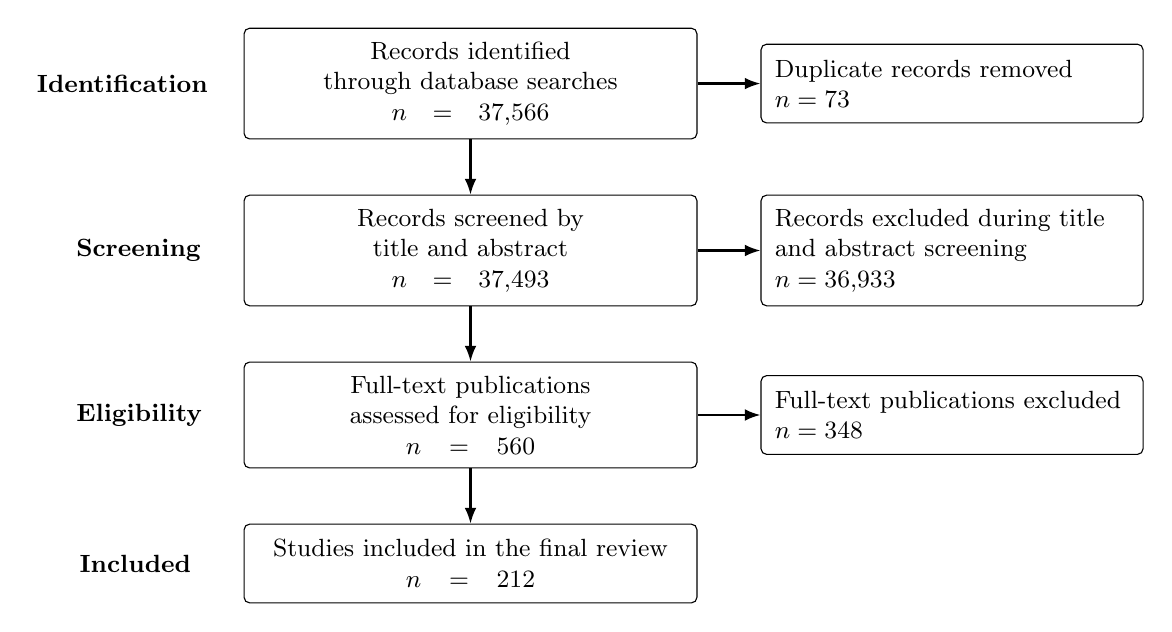
\begin{tikzpicture}[
node distance=7mm and 8mm,
box/.style={
draw,
rounded corners=2pt,
align=center,
text width=5.4cm,
minimum height=1cm,
inner sep=5pt,
font=\small
},
side/.style={
draw,
rounded corners=2pt,
align=left,
text width=4.5cm,
minimum height=1cm,
inner sep=5pt,
font=\small
},
stage/.style={
font=\small\bfseries,
align=center,
text width=1.5cm
},
arrow/.style={-{Latex[length=2mm]}, thick}
]

% Identification
\node[box] (identified) {
    Records identified through database searches\\
    \textbf{$n = 37{,}566$}
};

\node[side, right=of identified] (duplicates) {
    Duplicate records removed\\
    $n = 73$
};

% Screening
\node[box, below=of identified] (screened) {
    Records screened by title and abstract\\
    \textbf{$n = 37{,}493$}
};

\node[side, right=of screened] (excluded1) {
Records excluded during title and abstract screening\\
$n = 36{,}933$
};

% Eligibility
\node[box, below=of screened] (assessed) {
    Full-text publications assessed for eligibility\\
    \textbf{$n = 560$}
};

\node[side, right=of assessed] (excluded2) {
    Full-text publications excluded\\
    $n = 348$\\[2pt]
};

% Included
\node[box, below=of assessed] (included) {
    Studies included in the final review\\
    \textbf{$n = 212$}
};

% Main flow
\draw[arrow] (identified) -- (screened);
\draw[arrow] (screened) -- (assessed);
\draw[arrow] (assessed) -- (included);

% Exclusion flows
\draw[arrow] (identified) -- (duplicates);
\draw[arrow] (screened) -- (excluded1);
\draw[arrow] (assessed) -- (excluded2);

% PRISMA stages
\node[stage, left=10mm of identified] {Identification};
\node[stage, left=5mm of screened] {Screening};
\node[stage, left=5mm of assessed] {Eligibility};
\node[stage, left=5mm of included] {Included};

\end{tikzpicture}}
    \caption{PRISMA diagram of the study selection process}
    \Description{A flow diagram with four stages. Identification: 37,566 records found through database searches, of which 73 duplicates were removed. Screening: 37,493 records screened by title and abstract, of which 36,933 were excluded. Eligibility: 560 full texts assessed, of which 348 were excluded. Included: 212 studies in the final review.}
    \label{fig:prisma}
\end{figure}

\subsection{Quality Assessment}
\label{subsec:quality-assessment}

The selected studies were assessed with twelve quality assessment questions (QA1--QA12). The questions characterize the features and metrics used, how the experimental methods are reported, and how far each study investigates specific prediction settings and challenges. They cover feature characteristics and feature sets, semantic features, dataset descriptions, feature extraction and selection methods, validation procedures, feature combinations, online prediction, concept drift, effort-aware prediction, and cross-project prediction. Each question is answered on a three-point scale, with \textit{Yes} worth 1 point, \textit{Maybe} 0.5 points and \textit{No} 0 points. Table~\ref{tab:quality-assessment} lists the questions and the criteria for each answer.

\begin{table*}[t]
    \centering
    \footnotesize
    \setlength{\tabcolsep}{4pt}
    \caption{Quality assessment questions and scoring criteria}
    \label{tab:quality-assessment}
    \begin{tabular}{@{}p{0.04\textwidth}p{0.22\textwidth}p{0.22\textwidth}p{0.22\textwidth}p{0.22\textwidth}@{}}
        \toprule
        \textbf{ID} & \textbf{Question} & \textbf{Yes (1)} & \textbf{Maybe (0.5)} & \textbf{No (0)} \\
        \midrule
        QA1 & Does the study use features or metrics that leverage various characteristics of code changes for JIT defect prediction? & Uses features that capture at least two types of code-change characteristics (e.g., change size and diffusion). & Uses features that capture only one type of code-change characteristics (e.g., change size). & Uses no features that capture code-change characteristics (e.g., only developer-related features). \\
        QA2 & Does the study identify different sets of features used in JIT defect prediction? & Uses at least two different feature sets (e.g., AST-based features and the expert features of Kamei et al.). & Relies on a single feature set (e.g., the expert features of Kamei et al.). & Does not specify any feature set. \\
        QA3 & Does the study use semantic features that represent the underlying semantics of code changes? & Uses both expert and semantic features. & Uses only semantic features. & Uses only expert features. \\
        QA4 & Does the study sufficiently describe the datasets used in the experiments? & Provides sufficient details about the datasets used. & Uses some datasets without enough detail about their description. & Lacks a description of the datasets used. \\
        QA5 & Does the study report the methods and tools used for feature extraction and selection? & Clearly defines the methods and tools used for extracting and selecting features. & Uses external tools for extracting features. & Lacks the methodology and tools for extracting and selecting features. \\
        QA6 & Does the study validate the methods or tools used for feature extraction and selection? & Empirically validates the methods and tools used for feature extraction and selection. & Provides a validation scheme without any empirical work. & Does not validate the methods and tools used for feature extraction and selection. \\
        QA7 & Does the study evaluate the impact of different feature combinations on JIT defect prediction? & Examines the effect of different feature sets on JIT defect prediction performance. & Measures the effect of a single feature set on JIT defect prediction performance. & Reports performance for one feature set without characterizing any feature subsets. \\
        QA8 & Does the study investigate online JIT defect prediction? & Reports the performance of JIT defect prediction in an online setting. & Discusses online JIT defect prediction without relevant experiments. & Experiments only with a static set of features and does not discuss online prediction. \\
        QA9 & Does the study incorporate methods for detecting concept drift in online JIT defect prediction? & Examines several methods for detecting concept drift. & Uses a single method for detecting concept drift. & Does not discuss concept drift. \\
        QA10 & Does the study measure the performance of JIT defect prediction models in the presence of concept drift? & Reports changes in model performance in the presence of concept drift. & Provides some information on performance changes under concept drift, but not based on empirical work. & Provides no information on performance changes under concept drift. \\
        QA11 & Does the study investigate effort-aware JIT defect prediction? & Uses metrics to measure the performance of effort-aware JIT defect prediction. & Discusses such metrics but does not use them. & Does not mention metrics for effort-aware JIT defect prediction. \\
        QA12 & Does the study conduct experiments on cross-project JIT defect prediction? & Provides empirical results for cross-project JIT defect prediction. & Discusses cross-project performance without empirical investigation. & Does not discuss cross-project JIT defect prediction. \\
        \bottomrule
    \end{tabular}
\end{table*}

All twelve questions carry equal weight. The overall quality score of a study is the sum of its scores over QA1--QA12 and ranges from 0 to 12. Studies with an overall score below \tofill{3} (25\% of the maximum) were excluded under EC12. We chose a low threshold because QA8--QA12 address specialized settings, namely online prediction, concept drift, effort-aware prediction and cross-project prediction, that many otherwise relevant JIT studies do not investigate. The appraisal is therefore meant to remove only studies with minimal methodological and feature-related reporting, not to penalize studies for leaving out optional settings. The assessment results are also used to characterize the included studies in terms of feature-related practices, methodological reporting, and the prediction settings they investigate.

\subsection{Data Extraction and Synthesis}
\label{subsec:data-extraction}

A structured data extraction form is used to collect information from the full texts of the included studies. It extends the screening spreadsheet, which already holds the title, authors, publication year, link, search source, and inclusion or exclusion status of each study. The form captures the following items:

\begin{itemize}
    \item \textbf{Feature characteristics:} feature names, descriptions, categories, and calculation formulas (RQ1, RQ2).
    \item \textbf{Feature sets and extraction:} feature sets used, feature extraction methods and their descriptions, extraction tools, links to the tools, and descriptions of their functionality (RQ1, RQ2).
    \item \textbf{Predictive performance and experimental context:} performance metrics, reported effectiveness of feature sets, contribution of features or feature sets to predictive performance where reported, machine learning models, number and names of projects, their programming languages, and project categories (RQ3).
    \item \textbf{Concept drift:} whether concept drift is addressed, methods used to detect it, feature sets reported as robust to it, and differences in model performance associated with it (RQ4).
    \item \textbf{Prediction settings:} model performance in within-project and cross-project settings (RQ5).
\end{itemize}

The extracted information is synthesized with descriptive summaries and qualitative analysis. Descriptive summaries characterize the included studies, classify feature categories, and identify frequently reported features and temporal patterns. The qualitative synthesis compares feature definitions, extraction methods, experimental settings, predictive performance findings, and reported limitations.

The review synthesizes the predictive performance reported by primary studies and does not run new prediction experiments. Since studies differ in datasets, evaluation protocols and performance measures, their findings are interpreted in the context of their original experimental settings. Direct numerical comparisons are made only when they are methodologically justified. The synthesis also separates topics that primary studies explicitly investigate from those for which they report no evidence.

\section{Current Status and Next Steps}
\label{S:status}

This paper presented the protocol of an SLR on the feature sets used in JIT defect prediction and the outcome of its study selection. The search in six digital libraries returned 37,566 records, and 212 primary studies published between 2006 and 2025 were selected for the review. The next step is to extract data from the selected studies with the form described in Section~\ref{subsec:data-extraction} and to synthesize it to answer RQ1--RQ5. The expected outcome is a classification of the feature sets used in JIT defect prediction, a description of how they are extracted, a summary of the evidence on their predictive value, and an account of how primary studies deal with concept drift and with cross-project, online and effort-aware settings.

\bibliographystyle{ACM-Reference-Format}
\bibliography{references}

\end{document}
\endinput
